
\documentclass[border=8pt, multi, tikz]{standalone} 
\usepackage{import}
\subimport{../layers/}{init}
\usetikzlibrary{positioning}
\usetikzlibrary{3d} %for including external image 

\def\ConvColor{rgb:yellow,5;red,2.5;white,5}
\def\ConvReluColor{rgb:yellow,5;red,5;white,5}
\def\PoolColor{rgb:red,1;black,0.3}
\def\UnpoolColor{rgb:blue,2;green,1;black,0.3}
\def\FcColor{rgb:blue,5;red,2.5;white,5}
\def\FcReluColor{rgb:blue,5;red,5;white,4}
\def\SoftmaxColor{rgb:magenta,5;black,7}   
\def\SumColor{rgb:blue,5;green,15}

\newcommand{\copymidarrow}{\tikz \draw[-Stealth,line width=0.8mm,draw={rgb:blue,4;red,1;green,1;black,3}] (-0.3,0) -- ++(0.3,0);}

\begin{document}
\begin{tikzpicture}
\tikzstyle{connection}=[ultra thick,every node/.style={sloped,allow upside down},draw=\edgecolor,opacity=0.7]
\tikzstyle{copyconnection}=[ultra thick,every node/.style={sloped,allow upside down},draw={rgb:blue,4;red,1;green,1;black,3},opacity=0.7]

\node[canvas is zy plane at x=0] (input) at (-9,0,0) {
\includegraphics[width=12cm,height=12cm]{121_red.png}};

\node[canvas is zy plane at x=0] (input) at (-8,0,0) {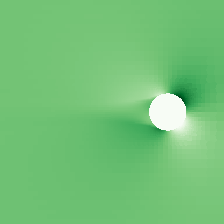
\includegraphics[width=12cm,height=12cm]{121_green.png}};

\node[canvas is zy plane at x=0] (input) at (-7,0,0) {
\includegraphics[width=12cm,height=12cm]{121_blue.png}};

\node[canvas is zy plane at x=0] (input) at (-3,0,0) {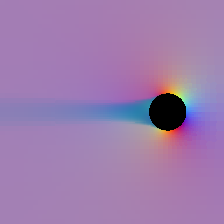
\includegraphics[width=12cm,height=12cm]{121_rgb.png}};

\pic[shift={(0,0,0)}] at (0,0,0) 
    {Box={
        name=conv1,
        caption= ,
        xlabel={{64, }},
        zlabel=112,
        fill=\ConvColor,
        height=56,
        width=16,
        depth=56
        }
    };

\pic[shift={ (0,0,0) }] at (conv1-east) 
    {Box={
        name=pool1,
        caption= ,
        fill=\PoolColor,
        opacity=0.5,
        height=14,
        width=2,
        depth=14
        }
    };

\pic[shift={(3,0,0)}] at (pool1-east) 
    {Box={
        name=conv2,
        caption= ,
        xlabel={{64, }},
        zlabel=56,
        fill=\ConvColor,
        height=14,
        width=16,
        depth=14
        }
    };

\draw [connection]  (pool1-east)    -- node {\midarrow} (conv2-west);

\pic[shift={(0,0,0)}] at (conv2-east) 
    {Box={
        name=conv3,
        caption= ,
        xlabel={{64, }},
        zlabel=56,
        fill=\ConvColor,
        height=14,
        width=16,
        depth=14
        }
    };

\pic[shift={(2,0,0)}] at (conv3-east) 
    {Box={
        name=conv4,
        caption= ,
        xlabel={{64, }},
        zlabel=56,
        fill=\ConvColor,
        height=14,
        width=16,
        depth=14
        }
    };

\draw [connection]  (conv3-east)    -- node {\midarrow} (conv4-west);

\pic[shift={(0,0,0)}] at (conv4-east) 
    {Box={
        name=conv5,
        caption= ,
        xlabel={{64, }},
        zlabel=56,
        fill=\ConvColor,
        height=14,
        width=16,
        depth=14
        }
    };

\pic[shift={ (0,0,0) }] at (conv5-east) 
    {Box={
        name=adaptive_pool,
        caption= ,
        fill=\PoolColor,
        opacity=0.5,
        height=3,
        width=2,
        depth=3
        }
    };

\pic[shift={(2,0,0)}] at (adaptive_pool-east) 
    {Box={
        name=fc1,
        caption= ,
        xlabel={{, }},
        zlabel=64,
        fill=\ConvColor,
        height=1,
        width=1,
        depth=20
        }
    };

\pic[shift={(1,0,0)}] at (fc1-east) 
    {Box={
        name=fc2,
        caption= ,
        xlabel={{, }},
        zlabel=6,
        fill=\ConvColor,
        height=1,
        width=1,
        depth=3
        }
    };

\draw [connection]  (adaptive_pool-east)    -- node {\midarrow} (fc1-west);

\draw [connection]  (fc1-east)    -- node {\midarrow} (fc2-west);

\end{tikzpicture}
\end{document}
